% The maximum length of a chess game under the FIDE Laws is 17,697 plies.
%
% Compile with: tectonic main.tex
%   (or latexmk -pdf main.tex; plain pdflatex twice also works --- the
%   bibliography is inline, so no BibTeX pass is needed)
\documentclass[11pt]{article}

\usepackage[T1]{fontenc}
\usepackage{amsmath,amssymb,amsthm}
\usepackage{array}
\usepackage{booktabs}
\usepackage{graphicx}
\usepackage{microtype}
\usepackage{xcolor}
\usepackage{xurl}
\usepackage[colorlinks=true,linkcolor=blue!50!black,citecolor=blue!50!black,urlcolor=blue!50!black]{hyperref}
\hypersetup{
  pdftitle={The maximum length of a chess game under the FIDE Laws is
    17,697 plies},
  pdfauthor={Junyeop Yim},
  pdfkeywords={chess, FIDE Laws of Chess, 75-move rule, longest chess
    game, computer-assisted verification},
}
\usepackage[margin=3.2cm]{geometry}

\newtheorem{theorem}{Theorem}[section]
\newtheorem{lemma}[theorem]{Lemma}
\newtheorem{proposition}[theorem]{Proposition}
\newtheorem{corollary}[theorem]{Corollary}
\theoremstyle{definition}
\newtheorem{definition}[theorem]{Definition}
\theoremstyle{remark}
\newtheorem{remark}[theorem]{Remark}
\newtheorem{convention}[theorem]{Convention}

\newcommand{\crit}{\mathrm{crit}}
\newcommand{\clock}{c}
\newcommand{\repo}[1]{\texttt{#1}}

\title{The maximum length of a chess game\\ under the FIDE Laws is 17{,}697 plies}
\author{Junyeop Yim\\[2pt]
  \small Department of Applied Mathematics, Kongju National University\\[1pt]
  \small\texttt{junyeobe0315@smail.kongju.ac.kr}}
\date{7~August 2026}

\begin{document}
\maketitle

\begin{abstract}
Under the FIDE Laws of Chess, which end a game automatically on a fivefold
repetition or when 75 moves by each player pass without a pawn move or a
capture, the length of a chess game is bounded. Labelle's analysis
\cite{labelle2015longest}, begun in 2015, identified the value $17{,}697$
plies ($8{,}848\tfrac12$ moves) by counting the clock-resetting moves
available, gave three-switch schedules and a complete generated game, and
left maximality a conjecture; Murphy \cite{murphy2020longest} later
published a separate complete construction of the same length, with a
counting ceiling of $17{,}699$. Neither source
excludes $17{,}698$ or $17{,}699$. We prove that the maximum is exactly
$17{,}697$. Writing $K$ for the number of critical segments of a game and
$S$ for the number of times the colour making the segment-ending moves
changes, every game satisfies $L \le 150K - S$; we show $K \le 118$, and
that $K = 118$ forces $S \ge 3$, which yields
$L \le 150 \cdot 118 - 3 = 17{,}697$. The argument is elementary, and every
finite case analysis it appeals to is machine-checked in a companion
repository, which also verifies the $17{,}697$-ply witness move by move and
re-decides the central case analysis by two independent mechanical methods.
\end{abstract}

\section{Introduction}\label{sec:intro}

How long can a game of chess be? Under earlier versions of the Laws the
question had no finite answer: the draw by threefold repetition and the
50-move rule must be \emph{claimed} by a player, so two cooperating players
could continue indefinitely. This changed on 1 July 2014, when FIDE
introduced two automatic termination rules \cite{fide2014laws}, retained in
the current Laws \cite{fide2023laws}: the game is drawn, without any claim, when the same
position occurs five times (Article~9.6.1), or when $75$ consecutive moves
by each player have been made without the movement of any pawn and without
any capture (Article~9.6.2) --- with the proviso that a checkmate delivered
by the final move takes precedence. Under these Laws the supremum of game
lengths is finite, and computing it exactly becomes a well-posed
combinatorial problem.

The question has a substantial informal history, and the value itself is
not new. For the older, claim-based 50-move setting --- under the
assumption that the claimable draws are in fact invoked --- Labelle
\cite{labelle2015longest} computed a maximum of $5{,}898\tfrac12$ moves.
For the modern automatic rules, the same analysis, maintained since 2015,
counts the clock-resetting moves available ($96$ pawn moves and $30$
captures, less $8$ moves that must be both), presents explicit schedules
--- due in part to contributors of the forum threads the page credits ---
realising all of them at the cost of three half-moves, and states, as a
belief supported by those constructions, that the maximum length is
$118 \times 75.0 - 3 \times 0.5 = 8{,}848\tfrac12$ moves; the page also
supplies a complete generated game of that length. Murphy
\cite{murphy2020longest} subsequently published a separate, hand-designed
complete game of $17{,}697$ plies ($8{,}848\tfrac12$ moves, ending in
checkmate on White's $8{,}849$th move) --- the witness verified in
Section~\ref{sec:witness} --- treating the exact maximum as open: his
counting ceiling admits $17{,}699$. Tromp's reference note
\cite{tromp-longest} records the value. Both sources thus establish the
lower bound $17{,}697$; neither excludes $17{,}698$ or $17{,}699$, and to
our knowledge no proof of optimality has been published. This paper
supplies one:

\begin{theorem}[Main theorem, proved as Theorem~\ref{thm:main}]
No legal chess game lasts more than $17{,}697$ plies, and the bound is
attained: the maximum length of a chess game under the FIDE Laws is
exactly $17{,}697$ plies.
\end{theorem}

Relative to the counting sketch of \cite{labelle2015longest}, the content
of the theorem is twofold. First, the count of $118$ is turned into an
upper bound over \emph{all} games: a game need not promote every pawn, so
the deduction of eight overlapping moves cannot be read off the intended
construction and must be derived --- Proposition~\ref{prop:pminuso}
couples the pawn-move and overlap counts through the number of resolved
files --- and the thirtieth capture interacts with the end of the game
(Lemma~\ref{lem:ct30}). Second, and this is the bulk of the paper, the
three half-move losses are proved unavoidable: no ordering of the critical
moves of any $118$-segment game achieves fewer than three colour changes
(Theorem~\ref{thm:s3}).

\paragraph{The shape of the proof.}
A \emph{critical move} --- a pawn move or a capture --- resets the 75-move
counter and is irreversible. Critical moves cut a game into \emph{segments},
each holding at most $149$ reversible plies plus the critical move that ends
it, so a game with $K$ segments has at most $150K$ plies; a parity argument
charges one further ply each time the \emph{colour} making the
segment-ending moves changes, giving $L \le 150K - S$
(Lemma~\ref{lem:decomposition}). Counting pawn moves and captures yields
$K \le 118$ (Theorem~\ref{thm:k118}), and $150 \cdot 118 - 1 = 17{,}699$ is
the ceiling of \cite{murphy2020longest}. The remaining two plies are
removed in Section~\ref{sec:switches}: a game attaining $K = 118$ is so
constrained --- all sixteen pawns must make six single-square moves each
and promote, and at least $29$ captures must occur --- that its critical
moves cannot be scheduled with fewer than three colour changes
(Theorem~\ref{thm:s3}). Four of the five candidate schedules are
eliminated by counting alone; the fifth is eliminated by a lemma about
pawns: \emph{while the enemy's pawns all stand on their home rank, an
advancing pawn stops four moves short of promotion}
(Lemma~\ref{lem:homerank}). Since $150 \cdot 117 = 17{,}550 < 17{,}697$,
games with $K \le 117$ are shorter still, and the theorem follows.

Nothing in the bound depends on how the game ends, which is why one argument
covers checkmate, the 75-move rule, fivefold repetition, stalemate and dead
positions alike.

\paragraph{Machine assistance, and what must be trusted.}
The proof is elementary and short enough to check by hand. Machine
assistance enters at clearly delimited points, all described in
Section~\ref{sec:methodology}: a handful of finite case analyses are
exhausted mechanically (each also proved by hand in the text); the
$17{,}697$-ply witness is verified ply by ply; and the central case analysis
of Section~\ref{sec:switches} is re-decided by two independent mechanical
methods, one a constraint solver and one solver-free, as a cross-check on
the human argument. A companion repository \cite{repo} contains all of this,
with a claims-to-code map reproduced in Appendix~\ref{app:claims}. The
trusted base is stated explicitly in Section~\ref{sec:trust}; it consists
of the FIDE Laws as summarised in Section~\ref{sec:setting} and, for the
mechanical checks only, the move generator of the \texttt{python-chess}
library \cite{pythonchess}.

\section{Setting, critical moves, and the segment decomposition}
\label{sec:setting}

\subsection{The rules assumed}\label{sec:rules}

A \emph{game} is a sequence of legal moves from the standard initial
position, played until a rule of the FIDE Laws \cite{fide2023laws} ends it.
We write $L$ for its length in \emph{plies} (single moves by one player) and
number plies from $1$; White plays the odd plies. The game-ending rules
relevant here are:
\begin{enumerate}
  \item \emph{Checkmate} (Art.~5.1.1) and \emph{stalemate} (Art.~5.2.1) end
    the game on the move that produces them.
  \item \emph{Dead position} (Art.~5.2.2): the game is drawn the moment a
    position arises from which no sequence of legal moves can lead to a
    checkmate by either side.
  \item \emph{Fivefold repetition} (Art.~9.6.1): the game is drawn, with no
    claim required, when the same position (same pieces on the same squares,
    same side to move, same castling and en passant possibilities, as in
    Art.~9.2.2) has occurred five times.\footnote{The 2014 formulation
    required the five occurrences to be consecutive; the requirement was
    removed in the 2017 revision \cite{fide2017laws}. The difference is
    immaterial here: the upper bound follows from the automatic
    75-move rule alone, and the verified witness never lets any position
    occur even three times (Section~\ref{sec:witness}).}
  \item \emph{Seventy-five--move rule} (Art.~9.6.2): the game is drawn, with
    no claim required, when at least $75$ consecutive moves by each player
    --- that is, $150$ consecutive plies --- have been played without any
    pawn move and without any capture. If the ply completing the $150$
    delivers checkmate, the checkmate stands.
\end{enumerate}
Draws by agreement, resignations, and the \emph{claimable} draws (threefold
repetition, Art.~9.2; the 50-move rule, Art.~9.3) are voluntary: players
maximising the length of a game simply never invoke them, so they play no
role in the maximisation. This is the setting of \cite{murphy2020longest}.

It is convenient to track the \emph{halfmove clock} $\clock(t)$: the number
of plies played since the most recent pawn move or capture (or since the
start of the game, if there has been none). Article~9.6.2 says precisely
that the game ends when $\clock$ reaches $150$, the ply that brings it there
being the last of the game, and being scored as mate if it mates.

\subsection{Critical moves and segments}

\begin{definition}[Critical move]\label{def:critical}
A \emph{critical move} is a pawn move or a capture. (En passant is both; a
promotion is a pawn move; castling is neither.) A \emph{quiet} move is a
move that is not critical.
\end{definition}

Critical moves are exactly the moves that reset the halfmove clock, and they
are irreversible: a pawn cannot retreat, and a captured man never returns.

\begin{definition}[Segments, endpoints, $K$, $T$]\label{def:segments}
Let $t_1 < t_2 < \dots < t_m$ be the plies of a game's critical moves. Set
$T = 1$ if quiet plies follow the last critical move (or if the game has
moves but no critical move at all), and $T = 0$ otherwise. The game's
\emph{endpoints} are
\[
  e_i = t_i \ (1 \le i \le m), \qquad e_{m+1} = L \text{ if } T = 1,
\]
together with the virtual endpoint $e_0 = 0$. The number of \emph{segments}
is $K = m + T$; segment $i$ consists of plies $e_{i-1}+1, \dots, e_i$.
Every ply lies in exactly one segment, and $e_K = L$.
\end{definition}

\begin{definition}[Switches $S$]\label{def:switches}
The \emph{colour} of an endpoint $e_i$ ($i \ge 1$) is the colour of the
player who played ply $e_i$ --- White if $e_i$ is odd, Black if even. By
convention the virtual endpoint $e_0 = 0$ is \emph{Black} (it has the parity
of a Black ply, and the game opens as if Black had just made a critical
move). The switch count is
\[
  S \;=\; \#\{\, i \in \{1,\dots,K\} : \text{colour}(e_i) \ne
  \text{colour}(e_{i-1}) \,\}.
\]
\end{definition}

\begin{lemma}[Segment decomposition]\label{lem:decomposition}
Every game satisfies
\[
  L \;=\; 150K - S - \sum_{i=1}^{K}\delta_i
  \qquad\text{with every } \delta_i \ge 0,
\]
where $\delta_i$ is the shortfall of segment $i$ from its target length
($150$ if endpoints $e_{i-1},e_i$ have the same colour, $149$ otherwise).
In particular $L \le 150K - S$.
\end{lemma}

\begin{proof}
Fix $i$ and consider the segment plies $e_{i-1}+1, \dots, e_i$. All of them
except possibly the last are quiet ($t_{i}$ is the next critical ply after
$t_{i-1}$; the terminal segment is entirely quiet). Suppose
$e_i - e_{i-1} \ge 151$. Then the $150$ plies
$e_{i-1}+1, \dots, e_{i-1}+150$ are all quiet, so after ply $e_{i-1}+150$
the halfmove clock reads $150$ and the game has ended there by
Article~9.6.2 (as a draw, or as the mate that takes precedence --- either
way it has ended), contradicting the existence of ply
$e_{i-1}+151 \le e_i \le L$. Hence $e_i - e_{i-1}\le 150$.

Plies alternate colours, so $e_i - e_{i-1}$ is even exactly when $e_i$ and
$e_{i-1}$ have the same colour; this is where the convention
$\text{colour}(e_0) = $ Black is used, $0$ having the parity of a Black
ply. A segment whose endpoints differ in colour therefore has odd length,
and being $\le 150$, has length $\le 149$. Summing the segment lengths
telescopes to $e_K - e_0 = L$ and yields the identity.
\end{proof}

\begin{remark}
The terminal quiet segment genuinely can reach $150$ plies: if the game
ends by the 75-move rule, the drawing ply is the $150$th quiet ply after
the last critical move and it \emph{is played}. Its parity then forces the
terminal endpoint to have the same colour as the previous one, consistent
with the accounting above. A terminal segment ending earlier --- by a quiet
checkmate, a stalemate, a fivefold repetition or a dead position --- is
only shorter.
\end{remark}

Counting critical moves by inclusion--exclusion, with $P$ the number of pawn
moves, $C$ the number of captures and $O$ the number of \emph{overlaps}
(moves that are both, i.e.\ diagonal pawn captures, en passant included),
\begin{equation}\label{eq:K}
  K \;=\; (P - O) + (C + T).
\end{equation}
The next two sections bound the two halves of \eqref{eq:K} separately.
Neither half refers to how the game ends.

\section{At most 118 critical segments}\label{sec:k118}

Throughout, we count over the $32$ \emph{units} that begin the game --- each
man followed through the whole game under promotion --- rather than over
piece types. A unit that begins as a pawn is still that unit after
promoting.

\begin{lemma}[Pawn basics]\label{lem:pawnbasics}
Each pawn makes at most $6$ pawn moves, so $P \le 96$. A pawn that makes
exactly $6$ pawn moves makes only single-square moves and promotes.
\end{lemma}

\begin{proof}
Every pawn move advances the pawn at least one rank toward promotion, and
there are six ranks between its home rank and the promotion rank. A pawn
making six moves therefore advances exactly one rank per move and finishes
on the promotion rank, where promotion is mandatory.
\end{proof}

\subsection{Origin pairs and the bound \texorpdfstring{$P - O \le 88$}{P - O <= 88}}

\begin{definition}[Origin pair, resolved file]\label{def:originpair}
The two pawns that begin on file $i$ (one White, one Black) are that file's
\emph{origin pair}. File $i$ is \emph{resolved} if at least one of those two
pawns makes a diagonal pawn move at some point in the game; otherwise it is
\emph{unresolved}. Write $f$ for the number of resolved files.
\end{definition}

A diagonal pawn move is the only way a pawn changes file, and it is always a
capture; so both pawns of an unresolved pair spend their entire lives on
file $i$.

\begin{lemma}[Unresolved pair cap]\label{lem:cap10}
The two pawns of an unresolved origin pair make at most $10$ pawn moves
combined, and $10$ is attained in a legal game.
\end{lemma}

\begin{proof}
Both pawns stay on file $i$. While both are on the board, the White pawn is
strictly below the Black one: neither can capture the other (a capture would
be diagonal), and neither can pass the other, since a single push onto an
occupied square is illegal and a double push may not jump over an occupied
square. So if White's pawn has advanced $a$ ranks and Black's $b$ ranks,
they stand on ranks $2+a < 7-b$, giving $a + b \le 4$; and since each pawn
move advances at least one rank, the two pawns have made at most $4$
combined moves while both are on the board. In particular neither pawn can
promote while the other is on the board, so at most one of the pair ever
promotes, and only after the other has been captured (necessarily by some
other unit).

When one pawn of the pair leaves the board its total contribution is frozen
at some $d \le 4$, and the survivor's lifetime total is at most $6$ by
Lemma~\ref{lem:pawnbasics}, for a combined total of at most
$d + 6 \le 10$.

Ten is attained: in
\[
  \text{1.\,Nf3 a6\; 2.\,Ng1 a5\; 3.\,Nf3 a4\; 4.\,Ng1 a3\; 5.\,Nxa3 Nc6\;
  6.\,Nc4 Rb8\; 7.\,a3 Nf6\; 8.\,a4 Ng8\;}
\]
\[
  \text{9.\,a5 Nf6\; 10.\,a6 Ng8\; 11.\,a7 Nf6\; 12.\,a8=Q Ng8}
\]
Black's a-pawn walks $a7$--$a3$ in four moves and is captured there by the
knight; White's a-pawn then walks the whole file and promotes, six more.
Neither pawn ever moved diagonally, so the a-file is unresolved throughout.
The sequence is a legal prefix rather than a completed game, but in any
legal completion neither count changes --- the survivor has promoted and
the other has been captured, so the pair makes no further pawn move and
the file stays unresolved --- so a completed legal game attains ten as
well. Figure~\ref{fig:cap10} shows the position after Black's fourth pawn
move and the final position of the sequence.
\end{proof}

\begin{figure}[t]
  \centering
  \begin{minipage}[t]{0.48\textwidth}
    \centering
    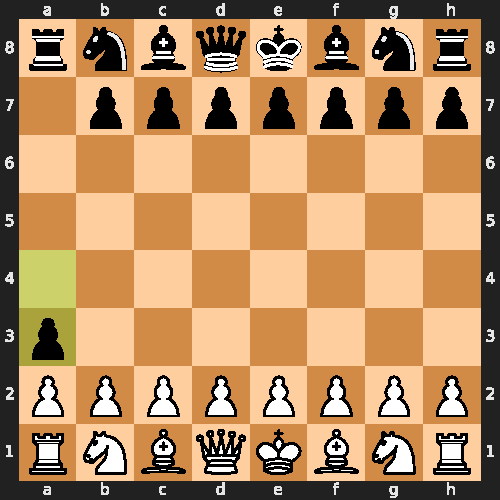
\includegraphics[width=0.82\linewidth]{figures/cap10-after}
    \par\smallskip (a)
  \end{minipage}\hfill
  \begin{minipage}[t]{0.48\textwidth}
    \centering
    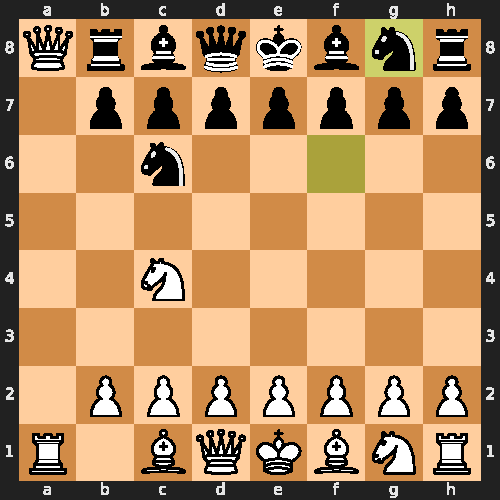
\includegraphics[width=0.82\linewidth]{figures/cap10-final}
    \par\smallskip (b)
  \end{minipage}
  \caption{The unresolved origin pair attaining ten combined pawn moves
  (Lemma~\ref{lem:cap10}). (a)~After 4\ldots a3: Black's a-pawn has made
  four moves and is captured on the next move by the b1-knight. (b)~The
  final position: White's a-pawn has walked the file and promoted, six
  further moves. Neither pawn ever left the a-file.}
  \label{fig:cap10}
\end{figure}

\begin{remark}\label{rem:cap10machine}
Both halves of the argument are additionally re-derived mechanically, by
exhausting a state space strictly more permissive than chess (turn order
ignored, no third unit blocking the file, either pawn removable at any
moment without cost); see Appendix~\ref{app:claims}. We record a caution
for anyone reproducing this bound: the first half of the argument alone ---
``two facing pawns cannot pass, so at most $4$'' --- is \emph{false} as a
cap, since it ignores that a captured pawn frees the survivor. A
constraint stronger than legality produces spurious impossibility results;
see Appendix~\ref{app:overconstraint}.
\end{remark}

\begin{lemma}[Overlap floor]\label{lem:overlapfloor}
$O \ge f$.
\end{lemma}

\begin{proof}
For each resolved file $i$ fix a witnessing diagonal pawn move; it is a
capture by a pawn whose \emph{origin} file is $i$. A pawn has one origin
file, so the witnessing moves of distinct resolved files have distinct
movers and are distinct moves, each of them an overlap.
\end{proof}

\begin{proposition}\label{prop:pminuso}
$P - O \le 88$, and equality forces $f = 8$, $P = 96$ and $O = 8$.
\end{proposition}

\begin{proof}
The eight origin pairs partition the sixteen pawns, so summing
Lemma~\ref{lem:cap10} over unresolved pairs and the trivial cap $12$ over
resolved pairs, and combining with Lemma~\ref{lem:pawnbasics},
\[
  P \;\le\; \min\bigl(96,\; 10(8-f) + 12f\bigr) \;=\; \min(96,\, 80 + 2f).
\]
With Lemma~\ref{lem:overlapfloor},
$P - O \le \min(96, 80+2f) - f$. For $f \le 7$ this is at most
$80 + 2f - f = 80 + f \le 87$; for $f = 8$ it is $96 - 8 = 88$. The maximum
over $f$ is therefore $88$, attained only at $f = 8$ with $P = 96$ and
$O = f = 8$.
\end{proof}

Maximising over $f$ is what makes Proposition~\ref{prop:pminuso} a statement
about all games rather than about games with eight overlaps; asserting
$O \ge 8$ outright would be circular, being true only \emph{because}
$K = 118$ forces every file to be resolved.

\subsection{The bound \texorpdfstring{$C + T \le 30$}{C + T <= 30}}

\begin{lemma}\label{lem:ct30}
$C + T \le 30$.
\end{lemma}

\begin{proof}
Only the $30$ non-king units can ever be captured, so $C \le 30$. If
$C \le 29$ then, since $T \le 1$, we get $C + T \le 30$. If $C = 30$, the
$30$th capture leaves the two kings alone on the board. King versus king is
a dead position --- no sequence of legal moves mates --- so by
Article~5.2.2 the game ends on that very ply; no quiet ply follows the last
critical move and $T = 0$, giving $C + T = 30$.
\end{proof}

This is the only place any dead-position reasoning enters the upper bound,
and king versus king is the one case where deadness is beyond dispute. The
two ways of reaching $30$ are worth displaying, because they explain why
draws do not outlast checkmates:
\[
  \underbrace{96 + 30 - 8 + 0}_{\text{all $30$ captured, no closing
  segment}} \;=\; \underbrace{96 + 29 - 8 + 1}_{\text{$29$ captured, one
  closing segment}} \;=\; 118 .
\]

\subsection{The bound \texorpdfstring{$K \le 118$}{K <= 118} and its equality case}

\begin{theorem}\label{thm:k118}
Every game has $K \le 118$. Moreover a game with $K = 118$ satisfies
\[
  f = 8, \qquad P = 96, \qquad O = 8, \qquad C + T = 30,
\]
so all sixteen pawns make six single-square pawn moves each and promote,
and $C \ge 29$.
\end{theorem}

\begin{proof}
By \eqref{eq:K}, Proposition~\ref{prop:pminuso} and Lemma~\ref{lem:ct30},
\[
  K = (P - O) + (C + T) \le 88 + 30 = 118 .
\]
Equality forces $P - O = 88$ and $C + T = 30$; the former pins
$(f, P, O) = (8, 96, 8)$ by the equality case of
Proposition~\ref{prop:pminuso}, and $P = 96$ makes every pawn's count
exactly $6$, whence Lemma~\ref{lem:pawnbasics} applies to each. Finally
$T \le 1$ gives $C \ge 29$.
\end{proof}

\begin{remark}
The uniqueness of the equality assignment is also verified by mechanical
enumeration of every $(f, P, O, C{+}T)$ the constraints admit at
$K = 118$ (there is exactly one) and at $K = 117$ (there are many, which is
what makes the pinning at $118$ informative). See
Appendix~\ref{app:claims}.
\end{remark}

Theorem~\ref{thm:k118} with $S \ge 1$ already gives Murphy's ceiling
$150 \cdot 118 - 1 = 17{,}699$. The next section removes the last two
plies.

\section{Games with 118 segments have at least three switches}
\label{sec:switches}

Throughout this section, fix a game with $K = 118$; by
Theorem~\ref{thm:k118} it has $P = 96$ --- \emph{every pawn makes exactly
six pawn moves} --- and $C \ge 29$. These two facts do all the work. We
emphasise at the outset that $S \ge 3$ is claimed \emph{only} under
$K = 118$; it is false in general (Remark~\ref{rem:notglobal}).

\subsection{Block shapes and the terminal seam}

The critical moves of a game, in order, form a sequence of coloured events
(the colour of a pawn move is the pawn's owner; the colour of a capture is
the capturer, i.e.\ the side that does \emph{not} own the victim). Group
maximal runs of equal colour into \emph{blocks}; the resulting alternating
sequence of block colours is the game's \emph{critical shape}. Counting the
virtual Black endpoint, an alternating sequence of $n$ blocks contributes
$n - 1$ switches if it opens with Black and $n$ if it opens with White.

The switch count $S$ of Definition~\ref{def:switches} is measured over all
$K$ endpoints, the last of which may be the terminal quiet endpoint rather
than a critical move. The two viewpoints line up in one step:

\begin{lemma}[Terminal seam]\label{lem:seam}
The endpoint sequence of a game is its critical-move sequence with, when
$T = 1$, one endpoint appended. Deleting a final element cannot increase
the number of adjacent unequal pairs, so if a game has $S \le 2$ then its
critical shape has at most $2$ switches as well.
\end{lemma}

\begin{proof}
Immediate. (In the companion repository the claim is additionally exhausted
over both readings of every alternating shape of up to twelve blocks.)
\end{proof}

A game with $K = 118$ has at least $117$ critical moves, so its critical
shape is nonempty; and a nonempty alternating shape with at most $2$
switches is one of exactly five:
\[
  \mathsf{B}, \qquad \mathsf{W}, \qquad \mathsf{BW}, \qquad \mathsf{WB},
  \qquad \mathsf{BWB},
\]
since $n$ blocks contribute at least $n - 1$ switches. We refute all five.
Each side has $15$ capturable units, of which exactly $7$ (queen, two
rooks, two bishops, two knights) did not begin as pawns; the count below is
over units, so a pawn-origin unit captured after promoting still counts
against the pawn origins.

\subsection{Four shapes are eliminated by counting}

\begin{proposition}[Single block]\label{prop:oneblock}
Shapes $\mathsf{B}$ and $\mathsf{W}$ are impossible at $K = 118$.
\end{proposition}

\begin{proof}
A pawn move is a critical move of the pawn's own colour. In a single-block
game only one colour makes critical moves, so only its eight pawns ever
move: $P \le 48 < 96$.
\end{proof}

\begin{proposition}[Two blocks]\label{prop:twoblocks}
Shapes $\mathsf{BW}$ and $\mathsf{WB}$ are impossible at $K = 118$.
\end{proposition}

\begin{proof}
Write the shape $(X, Y)$: every critical move of $X$ precedes every
critical move of $Y$. Since $Y$ captures only $X$'s units,
$C_Y \le 15$, so $C_X \ge C - 15 \ge 29 - 15 = 14$: the colour moving
first makes at least $14$ captures, all of them before $Y$ has made a
single critical move. Each victim is a $Y$ unit that, being dead before
every $Y$ critical move, never made a pawn move. At most $7$ of the victims
are non-pawn-origin units, so at least $7$ pawn-origin $Y$ units make no
pawn move at all, and
\[
  P \;\le\; 96 - 7 \cdot 6 \;=\; 54 \;<\; 96. \qedhere
\]
\end{proof}

Note that $Y$ may well have made \emph{quiet} moves in the meantime; the
argument only needs its critical moves to come later.

\subsection{The home-rank lemma}

One shape is not eliminated by counting alone; the following lemma closes
it.

\begin{lemma}[Home-rank lemma]\label{lem:homerank}
Fix colours $A$ (attacker) and $D$ (defender), and consider any position
reachable from the initial position by a sequence of moves satisfying
\begin{itemize}
  \item[\textup{(R1)}] every move by $D$ is quiet, and
  \item[\textup{(R2)}] no move by $A$ captures a $D$ pawn.
\end{itemize}
Then every square of $D$'s pawn home rank still holds the $D$ pawn that
started there; no $A$ pawn ever stands on that rank; and no $A$ pawn has
made more than four pawn moves.
\end{lemma}

\begin{proof}
We use the following facts about the rules, labelled for
Section~\ref{sec:methodology}, where their mechanical treatment is
described: \textup{[H0]} the initial position has eight pawns on each home
rank; \textup{[H1]} a legal move starts on a square holding a piece of the
side to move; \textup{[H2]} a move onto an occupied square is a capture of
an enemy piece standing there; \textup{[H3]} castling changes only
back-rank squares; \textup{[H4]} an en passant capture removes a pawn from
rank $4$ or rank $5$; \textup{[H5]} a move changes the occupancy of no
squares other than its origin and destination, the castling rook's two
squares, and the en passant victim's square; \textup{[H6]} a pawn move
advances the pawn exactly one rank, or exactly two from its own home rank
only.

\emph{Part 1: $D$'s home rank never changes.} Induction on moves, the base
case being [H0]. Let the invariant hold and let $m$ be a move permitted by
(R1), (R2). By [H5] it suffices to rule out each way $m$ could touch a
home-rank square. $m$ cannot \emph{start} there: the square holds a $D$
pawn, only $D$ may move it [H1], and that would be a pawn move, excluded by
(R1). $m$ cannot \emph{end} there: the square is occupied, so the move
would capture an enemy piece standing there [H2]; $D$ capturing is excluded
by (R1), and the occupant is a $D$ pawn, so $A$ capturing it is excluded by
(R2). Castling touches only back ranks [H3]. En passant removes a pawn from
rank $4$ or $5$ [H4], not from a home rank (and its victim would in any
case have just made a double push --- for a $D$ victim a pawn move,
excluded by (R1)).

\emph{Part 2: no $A$ pawn reaches $D$'s home rank.} Standing there requires
a move ending there, ruled out above.

\emph{Part 3: at most four moves.} By [H6] a pawn never moves backwards and
double-pushes only from its own home rank. By Part 2 an $A$ pawn never
occupies $D$'s home rank; nor the rank beyond it, which could only be
reached by a single step from $D$'s home rank or a double push from a rank
that is not the pawn's home rank. Its range is therefore the four ranks
between its own home rank and $D$'s, and each pawn move spends at least one
of them: at most four moves. (Four is attained, by four single pushes.)
\end{proof}

Figure~\ref{fig:homerank} shows a minimal instance of the confinement.

\begin{figure}[t]
  \centering
  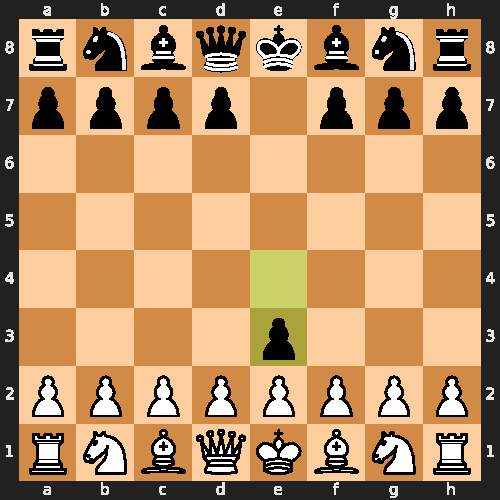
\includegraphics[width=0.42\textwidth]{figures/homerank}
  \caption{The home-rank lemma (Lemma~\ref{lem:homerank}), minimal
  instance. After 1.\,Nf3 e6\; 2.\,Ng1 e5\; 3.\,Nf3 e4\; 4.\,Ng1 e3,
  Black's pawn has made four moves and is confined: the square e2 holds a
  pawn that only White may move, which would violate (R1), and the
  captures on d2 and f2 are exactly what (R2) forbids.}
  \label{fig:homerank}
\end{figure}

\begin{proposition}[Three blocks]\label{prop:bwb}
Shape $\mathsf{BWB}$ is impossible at $K = 118$.
\end{proposition}

\begin{proof}
All of White's critical moves lie in the middle block. Let $\tau$ be the
ply of White's first critical move, and call the plies before $\tau$ the
\emph{first phase}. As in Proposition~\ref{prop:twoblocks}, Black captures
at most $15$ units, so White makes $C_W \ge 14$ captures, all in the middle
block; at least $14 - 7 = 7$ of the victims are pawn-origin Black units.

Fix such a victim. By Theorem~\ref{thm:k118} it makes exactly six pawn
moves, all before its capture. Its pawn moves are Black critical moves, and
Black critical moves at plies $> \tau$ belong to the third block, hence
come after \emph{every} White critical move --- in particular after the
capture, which is impossible for a dead unit. So all six of its pawn moves
occur in the first phase.

Now apply Lemma~\ref{lem:homerank} to the first phase with $A =$ Black,
$D =$ White. (R1) holds by the definition of $\tau$: every White move
before $\tau$ is quiet. (R2) holds because a White pawn captured before
$\tau$ would be dead before every White critical move and so would make
none of its six pawn moves, contradicting $P = 96$. The lemma caps every
Black pawn at four pawn moves in the first phase --- but each of the seven
victims needs six there. Even charging only the difference,
\[
  P \;\le\; 96 - 7 \cdot 2 \;=\; 82 \;<\; 96. \qedhere
\]
\end{proof}

The only escape the home-rank lemma allows --- capturing a way through the
home rank --- costs the captured pawn all six of its moves, which
Theorem~\ref{thm:k118} cannot spare. That is the entire content of clause
(R2) above.

\begin{theorem}\label{thm:s3}
Every game with $K = 118$ has $S \ge 3$.
\end{theorem}

\begin{proof}
Suppose $S \le 2$. By Lemma~\ref{lem:seam} the game's critical shape has at
most two switches, so it is one of the five shapes listed above; each is
refuted by Proposition~\ref{prop:oneblock}, \ref{prop:twoblocks} or
\ref{prop:bwb}.
\end{proof}

\begin{remark}\label{rem:notglobal}
$S \ge 3$ is conditional on $K = 118$, and only on it: every step above
runs on $P = 96$ and $C \ge 29$. It is plainly false in general. The
16-ply game \textup{1.\,Nf3 Nf6 2.\,Ng1 Ng8} repeated four times is legal
and ends in fivefold repetition of the initial position; it has no pawn
move and no capture, so $K = 1$ (the single closing segment), and its one
endpoint is a Black ply, matching the virtual Black opening: $S = 0$. This
costs nothing in Section~\ref{sec:main}: a game with $K \le 117$ forfeits
at least $150$ plies, more than any switch count could recover.
\end{remark}

\section{The main theorem}\label{sec:main}

\begin{theorem}\label{thm:main}
No legal chess game exceeds $17{,}697$ plies, and the game constructed in
\cite{murphy2020longest} attains this length. The longest chess game is
exactly $17{,}697$ plies --- $8{,}848$ full moves and one final White ply,
delivering checkmate on White's $8{,}849$th move.
\end{theorem}

\begin{proof}
Let a game have $K$ segments. If $K \le 117$ then by
Lemma~\ref{lem:decomposition} with the trivial $S \ge 0$,
\[
  L \;\le\; 150 \cdot 117 \;=\; 17{,}550 \;<\; 17{,}697 .
\]
If $K = 118$ --- the largest value Theorem~\ref{thm:k118} permits --- then
Theorem~\ref{thm:s3} gives $S \ge 3$, so
\[
  L \;\le\; 150 \cdot 118 - 3 \;=\; 17{,}697 .
\]
The bound is attained: Murphy's game is legal and $17{,}697$ plies long,
which we verify mechanically, ply by ply, in Section~\ref{sec:witness}.
\end{proof}

The two cases must be kept separate, because $S \ge 3$ is not available at
$K \le 117$ (Remark~\ref{rem:notglobal}); it is also not needed there,
since one whole segment outweighs any possible switch count.

\section{The witness}\label{sec:witness}

Among the published maximum-length games we verify the one constructed by
hand in \cite{murphy2020longest}; Labelle's page \cite{labelle2015longest}
supplies another, machine-generated. The companion repository \cite{repo}
contains an
independent verifier for it (built on the move generation of
\texttt{python-chess} \cite{pythonchess} and its own implementation of the
termination rules of Section~\ref{sec:rules}), together with a per-ply
trace. The verified facts:

\begin{itemize}
  \item The game is legal, $17{,}697$ plies long, and ends in checkmate,
    in the final position
    \texttt{3k4/3Q4/4K3/8/8/8/8/8} --- king and queen against king,
    Figure~\ref{fig:witnessfinal}.
  \item No automatic termination fires early. The halfmove clock stays
    below $150$ after every ply but the last; no position ever occurs even
    three times (the maximum multiplicity of any position over the whole
    game, under the identity of Article~9.2.2, is \emph{two}), so
    fivefold repetition is never approached; no stalemate occurs.
  \item No position of the game is dead, by an argument that needs no
    material test: from every position, the remaining moves of the game
    are themselves a legal series ending in checkmate, and a position from
    which checkmate is reachable is precisely what Article~5.2.2 does not
    end. The verifier checks the legality of those suffixes; its
    material-based deadness test is not load-bearing here (see
    Section~\ref{sec:trust}).
  \item The final ply is a quiet checkmate played with the halfmove clock
    at exactly $150$: the game ends on the precedence clause of
    Article~9.6.2. Its length is insensitive to that clause --- under
    either reading the $17{,}697$th ply is played and the game ends on it;
    the clause decides only whether the result is a win or a draw.
  \item The profile is the equality case of Theorem~\ref{thm:k118}:
    $117$ critical moves plus a closing segment ($K = 118$), with
    $P = 96$ (each of the sixteen pawns makes exactly six pawn moves),
    $C = 29$, $O = 8$ (every file resolved), $T = 1$. The endpoint colour
    sequence has shape $\mathsf{BWBW}$, so $S = 3$, and the decomposition
    of Lemma~\ref{lem:decomposition} closes exactly:
    $115$ segments of $150$ plies, $3$ segments of $149$ (one per switch),
    and $\sum_i \delta_i = 0$:
    \[
      17{,}697 \;=\; 150 \cdot 118 - 3 - 0 .
    \]
\end{itemize}

\begin{figure}[t]
  \centering
  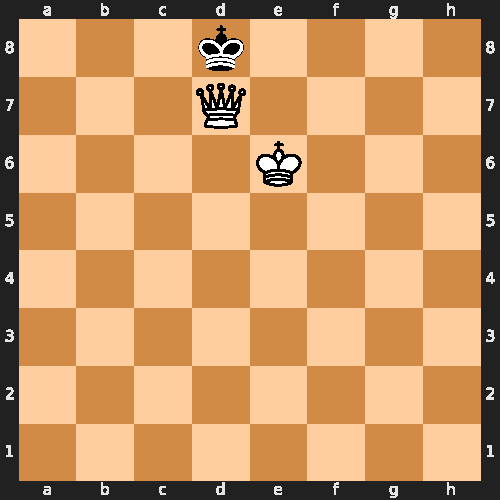
\includegraphics[width=0.42\textwidth]{figures/witness-final}
  \caption{The final position of the witness, after ply $17{,}697$:
  checkmate, delivered with the halfmove clock at exactly $150$.}
  \label{fig:witnessfinal}
\end{figure}

Improving on the witness would require eliminating a colour switch rather
than packing segments more tightly: it already fills every segment, and
its three lost plies are exactly the three boundaries
Theorem~\ref{thm:s3} proves unavoidable. The repository also \emph{rebuilds} a different game of
the same length --- same $118$ critical moves, freshly generated quiet
filler; $17{,}032$ of the $17{,}697$ plies differ --- and verifies it the
same way, so attainment does not rest on a single artefact.

\section{Verification methodology}\label{sec:methodology}

The proof above is a hand argument, and we intend it to be checkable
entirely by hand. This section records what was additionally checked by
machine, and what a sceptical reader must trust. The companion repository
\cite{repo} packages all of it; Appendix~\ref{app:claims} maps each claim
to the code that checks it, every check re-runs from a
byte-for-byte--reproducible certificate, and
Appendix~\ref{app:overconstraint} analyses the failure mode specific to
this style of checking, with the three instances repaired during the
work.

\subsection{Finite checks}\label{sec:finite}

The following case analyses, each also proved in the text, are exhausted
mechanically:
the unresolved-pair cap of Lemma~\ref{lem:cap10}, over a state space
strictly more permissive than chess (Remark~\ref{rem:cap10machine});
the impossibility of two facing pawns passing each other on a file;
the uniqueness of the equality assignment of Theorem~\ref{thm:k118};
the terminal seam of Lemma~\ref{lem:seam} over every alternating shape of
up to twelve blocks;
and, for Lemma~\ref{lem:homerank}, the obligations [H0] (16 squares of the
initial position), [H3] (all four castling moves) and [H4] (all 28 en
passant configurations), which have finitely many instances and are settled
outright.

The remaining obligations [H1], [H2], [H5], [H6] are universally
quantified over all positions, so no enumeration can settle them; they are
read off the Laws \cite{fide2023laws}, and the repository checks them
against a large randomised corpus of positions. That corpus check tests
that the move generator we rely on implements those four rules correctly
--- it is a check on the tooling, not on the mathematics.

In addition, the home-rank lemma was attacked adversarially before it was
proved: a search playing real chess under (R1), (R2) --- with a control run
confirming the search can break through once the restrictions are lifted
--- examined every legal attacker move at every position visited
($4{,}430{,}269$ moves across $90{,}779$ positions, seeded and
reproducible) and found no pawn reaching the defended home rank and no en
passant capture ever available. The search is evidence; the induction of
Lemma~\ref{lem:homerank} is the argument the evidence was for.

\subsection{Two independent mechanical decisions of
Theorem~\ref{thm:s3}}\label{sec:crosschecks}

To reduce the risk of an undetected error in the hand argument of
Section~\ref{sec:switches}, the question ``does any shape with $S \le 2$
admit $K = 118$?'' is re-decided mechanically by two further methods: a
CP-SAT constraint model \cite{ortools}, and a solver-free arithmetic
checker that declares its own constants and decides the same question by
direct enumeration. Their verdicts carry weight only under a precisely
stated soundness property, which we give for the constraint model; the
arithmetic checker imposes aggregated forms of the same conditions, each
likewise a necessary condition of legality.

Fix an alternating block shape $\sigma$, an ending
$e \in \{\text{checkmate}, \text{draw}\}$, and a target $k$. The model
$M(\sigma, e, k)$ is a finite system of constraints over bounded integer
variables: per-pawn pawn-move counts in each block of the pawn's colour,
with a per-pawn total of at most six; per-unit capture indicators, each
captured unit assigned a death block of the enemy colour, a captured
pawn-origin unit making no pawn move in any later block; capture, overlap
and closing-segment totals with the coupling of Proposition~\ref{prop:pminuso} imposed through
a free resolved-file count; the cap of Lemma~\ref{lem:homerank} on
opening-block pawn moves, imposed only while no enemy pawn has been
captured in that block; for $e = \text{checkmate}$, the requirement that
the side owning the final block retain at least one non-king unit; and the
requirement that the totals compose to $k$ as in \eqref{eq:K}.

\emph{Soundness property.} Let $G$ be a legal game with $K(G) = k$ whose
endpoint sequence has shape $\sigma$, and set $e$ to checkmate if $G$ ends
in mate and to draw otherwise. Then the observed values of $G$ --- its
per-pawn, per-block move counts, its capture blocks, and its totals ---
satisfy every constraint of $M(\sigma, e, k)$. This holds because each
constraint is individually a necessary condition of legality; the
constraint-by-constraint argument is recorded in the repository's model
audit, and the attribution of the mating side to the final block is sound
precisely because shapes are sequences of segment endpoints
(Definition~\ref{def:segments}), the mate being the last endpoint.
Consequently, if $M(\sigma, e, 118)$ is infeasible for both values of $e$,
then no legal game with endpoint shape $\sigma$ attains $K = 118$. No
claim is made in the converse direction: a satisfying assignment need not
correspond to any legal game, and no conclusion of this paper rests on a
feasibility verdict.

Coverage is finite. An alternating shape of $n \ge 5$ blocks has $S \ge 4$
by the block count of Section~\ref{sec:switches}, so the sixteen decided
instances --- the eight shapes of at most four blocks, under both endings
--- include every shape relevant to Theorem~\ref{thm:s3}. CP-SAT decides
each finite instance exactly; a solver timeout is surfaced as an error and
never reported as infeasibility. The results, identical under both
endings: every shape with $S \le 2$ is infeasible, in agreement with the
counting proof, and the feasible shapes are exactly $\mathsf{BWBW}$ and
$\mathsf{WBWB}$. Thus every feasible shape has $S \ge 3$; the converse
fails and is not claimed --- $\mathsf{WBW}$, with $S = 3$, is also
infeasible, a verdict beyond what Theorem~\ref{thm:s3} requires and in no
tension with it, since infeasibility only ever removes games. Removing
the home-rank constraint changes exactly $\mathsf{BWB}$ and
$\mathsf{WBW}$ from infeasible to feasible and leaves every other verdict
unchanged, confirming that the lemma carries precisely the case
Proposition~\ref{prop:bwb} assigns to it and that no other refutation of
Section~\ref{sec:switches} depends on it.

The soundness property cannot be established by testing, but violations of
it can be witnessed: the constraint model accepts the exact assignment
induced by the witness game of Section~\ref{sec:witness}, both deciders
return feasible for its endpoint shape $\mathsf{BWBW}$, and
Appendix~\ref{app:overconstraint} records three constraints that were, at
some stage of this work, stronger than legality --- each found by the
constraint-by-constraint argument, none surviving in the reported
verdicts.

\subsection{The trusted base}\label{sec:trust}

A reader who checks the hand proof of
Sections~\ref{sec:setting}--\ref{sec:main} and re-runs the repository must
still trust the following.
(i) The summary of the Laws in Section~\ref{sec:rules}, in particular that
Articles 9.6.1--9.6.2 end games automatically and that mate takes
precedence on the final ply --- the witness's length, though not its
result, is insensitive to the precedence clause.
(ii) The move generation of \texttt{python-chess} \cite{pythonchess}
(version pinned in the repository), which underlies the witness
verification and the corpus checks of Section~\ref{sec:finite}; the
obligations [H1], [H2], [H5], [H6] are facts about chess that we verify
the library respects, not facts we derive from it. The witness is an
artefact produced by others \cite{murphy2020longest} and accepted by our
verifier, which separates producer from judge; an additional verification
under an independently implemented move generator would shrink this trust
further and is noted as future work.
(iii) That the dead-position rule never shortens the witness: this needs
no decision procedure for Article~5.2.2, only the observation of
Section~\ref{sec:witness} that a game ending in mate contains no dead
position. The upper bound uses deadness once, for king versus king
(Lemma~\ref{lem:ct30}), where it is beyond dispute; everywhere else,
ignoring dead positions only lengthens hypothetical games, which is the
safe direction for an upper bound.
The counting proof itself is not formalised in a proof assistant; a
formalisation (with the human text as its blueprint) is natural future
work.

\section*{Acknowledgements}

This work exists because Tom Murphy VII built a $17{,}697$-ply game and
asked, in the title of \cite{murphy2020longest}, whether it is the
longest; the answer is yes. The structure of that answer --- $118$
clock-resetting moves, three unavoidable half-move losses --- was
identified years earlier by Fran\c{c}ois Labelle
\cite{labelle2015longest}, together with the forum contributors his page
credits.

This work was carried out independently, outside any research group and
without funding.

The board diagrams were rendered with python-chess \cite{pythonchess};
the piece images are by Colin~M.\,L.~Burnett, triple-licensed under the
GFDL, BSD and GPL, and are used here under the BSD option with this
attribution.

\appendix

\section{Claims-to-repository map}\label{app:claims}

The companion repository \cite{repo} verifies the following claims
mechanically. The table names each statement and the routine that decides
it; module paths, the tests that pin each claim, invocation commands,
expected outputs and measured runtimes are catalogued in the repository's
top-level \texttt{CLAIMS.md}, and a certificate directory records every
verdict together with a hash of every artefact, re-derivable byte for
byte from a clean checkout.

\begin{center}
\small
\begin{tabular}{@{}ll@{}}
\toprule
Statement & Deciding routine \\
\midrule
Lemma~\ref{lem:cap10}, cap exhausted over a relaxation &
  \texttt{check\_origin\_pair\_cap} \\
Lemma~\ref{lem:cap10}, cap attained legally &
  the 24-ply legal prefix, replayed \\
Lemma~\ref{lem:cap10}, facing pawns cannot pass &
  \texttt{check\_file\_lemma} \\
Proposition~\ref{prop:pminuso}, maximiser unique at $f = 8$ &
  \texttt{pawn\_minus\_overlap\_bound} \\
Theorem~\ref{thm:k118}, equality assignment unique &
  \texttt{equality\_witnesses} \\
Lemma~\ref{lem:seam}, over all shapes of $\le 12$ blocks &
  \texttt{check\_terminal\_endpoint\_free} \\
Lemma~\ref{lem:homerank}, obligations [H0]--[H6] &
  \texttt{invariant.verify} \\
Lemma~\ref{lem:homerank}, adversarial search &
  \texttt{adversary.audit} \\
Section~\ref{sec:switches}, the five refutations &
  \texttt{switch\_lower\_bound} \\
Section~\ref{sec:crosschecks}, sixteen instances and the ablation &
  \texttt{solve}, \texttt{analyse} \\
Section~\ref{sec:witness}, witness verification &
  \texttt{verifier} \\
Section~\ref{sec:witness}, the rebuilt second witness &
  \texttt{pad\_skeleton} \\
Appendix~\ref{app:overconstraint}, regression pins &
  the repository test suite \\
certificate reproducibility &
  \texttt{certify}, \texttt{check\_certificate} \\
\bottomrule
\end{tabular}
\end{center}

The repository version corresponding to this paper is tag
\texttt{v1.0.0}, cited in \cite{repo} together with the archival DOI of
that release's Zenodo deposit.

\section{Over-constraint: three repaired instances}
\label{app:overconstraint}

Impossibility checking over necessary conditions has one failure mode
that cannot be detected from its verdicts alone: a constraint stronger
than legality produces spurious infeasibility, indistinguishable from a
correct refutation. Three such constraints were introduced and later
repaired during this work. They are recorded here because the record
bears on the auditing standard applied to the surviving constraints, and
because none of the three was found by testing --- each was found by the
constraint-by-constraint argument of
Section~\ref{sec:crosschecks}, which is the only mechanism that can find
them.

\emph{First instance.} An early version capped an unresolved origin pair
at $4$ combined pawn moves --- the first half of the proof of
Lemma~\ref{lem:cap10} mistaken for the whole. The cap is refuted by a
legal $15$-ply sequence ending with 8.\,a5, in which a bishop captures
one pawn of the pair and the survivor advances freely
(Figure~\ref{fig:overconstraint}(a)). The corrected cap of $10$ weakens the
coupling of Proposition~\ref{prop:pminuso} at every $f$ while leaving its
maximum of $88$ unchanged, so Theorem~\ref{thm:k118} was unaffected; the
margins by which the five shapes of Section~\ref{sec:switches} fail had,
however, been overstated, and were re-derived.

\emph{Second instance.} The model's checkmate branch once required the
mated side to lose all fifteen of its capturable units. The condition
does hold at $K = 118$, where it follows from $C + T = 30$, but it is not
a consequence of checkmate --- a scholar's-mate game refutes it --- and
imposed unconditionally it excluded legal games at other targets. It was
weakened to the condition stated in Section~\ref{sec:crosschecks}, which
is all that checkmate implies.

\emph{Third instance.} Reading the final block of a shape as the mating
side is sound over sequences of segment endpoints and unsound over
critical-move sequences alone: a quiet mate can be delivered by the
colour that made no critical move last, and an explicit $76$-ply legal
game realises the gap --- its critical actors form
$(\mathsf{B}, \mathsf{W})$ while Black delivers the mate
(Figure~\ref{fig:overconstraint}(b)). The convention
had been applied consistently but stated nowhere, and one description of
the model used the incorrect reading. The convention is now explicit in
the soundness property of Section~\ref{sec:crosschecks}, resting on
Definition~\ref{def:segments}, and the witnessing game is pinned as a
regression.

In all three cases the sixteen decided instances were re-derived after
repair and no verdict changed. For the second and third instances this is
provable in retrospect: the offending constraint is derivable at
$K = 118$ (second), and the draw instances, which carry no mating-side
condition at all, are infeasible for the same six shapes (third).

\begin{figure}[t]
  \centering
  \begin{minipage}[t]{0.48\textwidth}
    \centering
    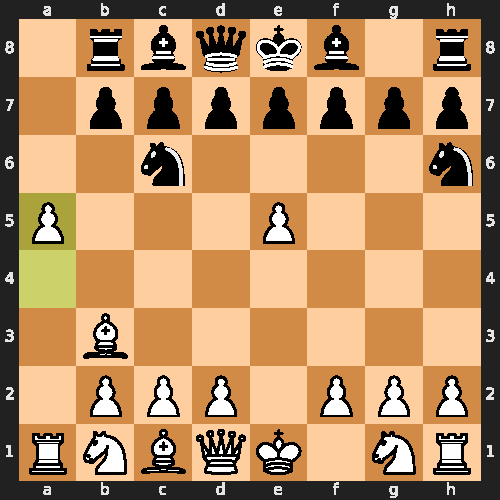
\includegraphics[width=0.82\linewidth]{figures/cap4-false}
    \par\smallskip (a)
  \end{minipage}\hfill
  \begin{minipage}[t]{0.48\textwidth}
    \centering
    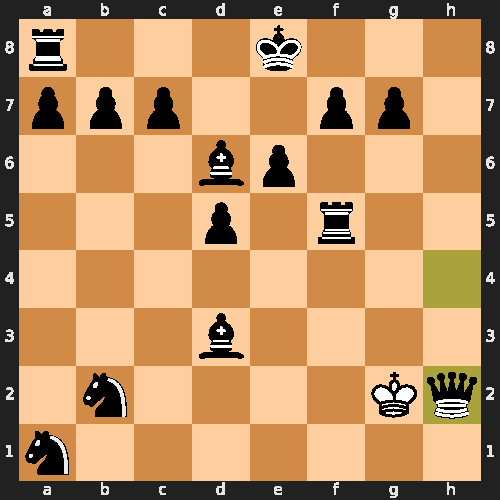
\includegraphics[width=0.82\linewidth]{figures/quiet-mate}
    \par\smallskip (b)
  \end{minipage}
  \caption{The two witnessed instances of Appendix~\ref{app:overconstraint}.
  (a)~First instance, after 8.\,a5: the a-file's origin pair has made five
  combined pawn moves against a cap that asserted four, neither pawn ever
  leaving the file. (b)~Third instance, the final position of the
  $76$-ply game: every Black critical move precedes White's single one
  (the king's capture on g2), and Black has just delivered a quiet mate.}
  \label{fig:overconstraint}
\end{figure}

\begin{thebibliography}{9}

\bibitem{labelle2015longest}
F.~Labelle.
\newblock The longest possible chess game, and bounds on the number of
  possible chess games.
\newblock Web page, created 14~November 2015, last updated 17~October
  2020, accessed August 2026.
\newblock \url{https://wismuth.com/chess/longest-game.html}; archived at
  \url{https://web.archive.org/web/20260806171843/https://wismuth.com/chess/longest-game.html}.

\bibitem{murphy2020longest}
T.~Murphy~VII.
\newblock Is this the longest Chess game?
\newblock In \emph{A Record of the Proceedings of SIGBOVIK 2020}, April
  2020.
\newblock \url{http://tom7.org/chess/longest.pdf}.

\bibitem{fide2014laws}
FIDE.
\newblock \emph{Laws of Chess: for competitions starting from 1 July 2014
  till 30 June 2017}, FIDE Handbook E/01.
\newblock \url{https://handbook.fide.com/chapter/E012014}.

\bibitem{fide2017laws}
FIDE.
\newblock \emph{Laws of Chess: taking effect from 1 July 2017}, FIDE
  Handbook E/01.
\newblock \url{https://handbook.fide.com/chapter/E012017}.

\bibitem{fide2023laws}
FIDE.
\newblock \emph{FIDE Laws of Chess}, FIDE Handbook E/01, in force from
  1~January 2023.
\newblock \url{https://handbook.fide.com/chapter/E012023}.

\bibitem{tromp-longest}
J.~Tromp.
\newblock The longest chess game.
\newblock Web note, \url{https://tromp.github.io/chess/longest.html},
  accessed August 2026; archived at
  \url{https://web.archive.org/web/20260806171910/https://tromp.github.io/chess/longest.html}.

\bibitem{pythonchess}
N.~Fiekas.
\newblock python-chess: a chess library for Python, version 1.11.2.
\newblock \url{https://github.com/niklasf/python-chess}.

\bibitem{ortools}
L.~Perron and F.~Didier.
\newblock CP-SAT solver, Google OR-Tools.
\newblock \url{https://developers.google.com/optimization/cp/cp_solver}.

\bibitem{repo}
J.~Yim.
\newblock Companion repository for ``The maximum length of a chess game
  under the FIDE Laws is 17,697 plies''.
\newblock \url{https://github.com/junyeobe0315/long_chess}, 2026.
\newblock Version \texttt{v1.0.0}, archived at
  \url{https://doi.org/10.5281/zenodo.21828026}.

\end{thebibliography}

\end{document}
